Este capítulo tem como objetivo apresentar a metodologia da avaliação de desempenho das diferentes bibliotecas de ML selecionadas.

\section{Metodologia}

A avaliação de desempenho seguirá a abordagem sistemática para a realização de avaliações de desempenho, proposta por Raj Jain e descrita na seção \ref{performance_analysis_theory}.

O objetivo desta análise consiste em comparar diversas bibliotecas de aprendizagem de máquina, utilizadas em programas Java e Python, de modo a escolher a melhor alternativa no quesito velocidade na realização de inferência de modelos de ML.

O sistema a ser avaliado consiste de um módulo de programação, programado em Python ou Java de acordo com a análise realizada no capítulo \ref{chapter-literature}, que fornece um serviço de inferência de modelos pré-treinados e carregados em memória, onde ao receber dados de entrada de um tipo especificado pelo modelo, executa o modelo com a entrada recebida e retorna o valor inferido do modelo.

Nesta análise, erros e falhas durante a execução do serviço não serão consideradas. Em cada execução do serviço, serão registrados o tempo de total de execução e o resultado da mesma. As alternativas serão comparadas de acordo com a métrica principal de desempenho: o tempo de execução por chamada; devido à necessidade de diminuir o tempo de inferência dos modelos como elencado na seção \ref{3-motivation}. Além disso, os resultados de cada alternativa serão comparados entre si para verificar se há perda ou ganho de precisão do modelo de acordo com o formato em que se encontra serializado e a biblioteca de ML utilizada para a execução.

Diversos parâmetros influenciam o desempenho do sistema:

\begin{itemize}
  \item Velocidade da CPU da máquina;
  \item Velocidade e funcionalidades da GPU da máquina, em execuções de modelo que utilizam a GPU para inferência;
  \item Formato de serialização em que o modelo está salvo;
  \item Biblioteca utilizada para a execução do modelo;
  \item Uso ou não da GPU para a execução do modelo;
  \item Número, tamanho e valor dos dados de entrada de uma execução de modelo;
  \item Número e tamanho dos dados de saída de uma execução de modelo;
  \item Ambiente de execução, ou \textit{runtime environment} em que o programa é executado.
\end{itemize}

Dentre estes parâmetros, foram selecionados 3 parâmetros como fatores:

\begin{itemize}
  \item Ambiente de execução. Serão executados programas escritos em Python, executados com \textit{runtime} Python 3.8.5, e em Java, executados com \textit{runtime} OpenJDK 11.0.7+10.
  \item Biblioteca utilizada para a execução do modelo. Como avaliado na seção \ref{chapter-literature}, serão consideradas as bibliotecas ONNX Runtime, Tensorflow Lite, TensorFlow, OpenCV e Deeplearning4j.
  \item Uso de GPU. Haverão experimentos com uso de GPU na execução dos modelos e sem o uso de GPU.
  \item Formato de serializção em que o modelo está salvo. Onde será utilizado o arquivo original do modelo em formato HDF5 e outros arquivos convertidos quando necessário, em formatos ONNX e tflite.
\end{itemize}

A medição será a técnica de avaliação de desempenho escolhida pelo fato do autor se especializar em programação. Assim, as diferentes alternativas de sistemas a serem comparadas serão implementadas e instrumentadas na execução da análise de desempenho, sendo cada uma das implementações um programa desenvolvido em Python ou Java.

Para a simulação, um classificador de estratégias de RSA em EONs, baseado em \textit{deep learning}, será utilizado para comparação. Este modelo recebe como entrada o estado de uma EON e tem como saída a classificação da estratégia RSA em utilização, de acordo com o estado. O modelo possui como saída uma classificação da estratégia de alocação identificada pelo estado como ruim, média ou boa.

A carga de trabalho é formada por 97301 diferentes estados de rede coletados de execuções reais do ONS, sendo cada estado representado por uma matriz de 86 linhas e 320 colunas, a representação da topologia USANet com 24 nós e 86 enlaces em que cada enlace contém 320 \textit{slots}.

Os experimentos a serem realizados consistem em um desenho fatorial fracionário, onde diversas combinações foram descartadas por incompatibilidade de fatores, como o uso de Deeplearning4j em Python, ou motivos diversos detalhados no capítulo \ref{chapter-literature}. Assim, serão realizadas as seguintes combinações de experimentos:

\begin{itemize}
  \item Java, Deeplearning4j, sem GPU, modelo original no formato HDF5 (TensorFlow);
  \item Java, Deeplearning4j, com GPU, modelo original no formato HDF5 (TensorFlow);
  \item Java, ONNX Runtime, sem GPU, modelo convertido para o formato ONNX;
  \item Java, ONNX Runtime, com GPU, modelo convertido para o formato ONNX;
  \item Python, OpenCV, sem GPU, modelo convertido para o formato ONNX;
  \item Python, Tensorflow Lite, sem GPU, modelo convertido para o formato TFLite;
  \item Python, Tensorflow, sem GPU, modelo original no formato HDF5 (TensorFlow);
  \item Python, Tensorflow, com GPU, modelo original no formato HDF5 (TensorFlow);
  \item Python, ONNX Runtime, sem GPU, modelo convertido para o formato ONNX;
  \item Python, ONNX Runtime, com GPU, modelo convertido para o formato ONNX.
\end{itemize}

Cada elemento da carga de trabalho foi executado 5 vezes por todas as combinações de simulação, sendo selecionada a mediana de cada uma destas 5 execuções com o objetivo de remover ruídos arbitrários causados pela máquina durante a execução.

\section{Ambiente de Medição}

Para a realização das medições, 10 programas foram desenvolvidos considerando todas as combinações de linguagens (Java e Python), bibliotecas (ONNX Runtime, Tensorflow Lite, Tensorflow, OpenCV e Deeplearning4j) e o uso ou não da GPU para execução de modelos. Estes programas realizam o mesmo conjunto de tarefas: 1. inicializar o sistema ao carregar o modelo; 2. inicializar procedimentos necessários para a execução da carga de trabalho; 3. carregar a carga de trabalho usada como entrada do modelo; 4. realizar as chamadas de serviço com as entradas carregadas para executar o modelo.

Cada programa trata de medir apenas o intervalo de tempo em que a execução do modelo ocorre. A execução de um dos programas foi orquestrada por \textit{scripts} auxiliares feitos em Python, responsáveis por instalar dependências, e executar os programas de simulação.

As simulações foram realizadas em uma máquina com processador Intel Core i3-8100, placa de vídeo GeForce RTX 2060 e memória RAM de 32 GB (2x16GB 3000Mhz DDR4). O código-fonte dos programas de simulação e de programas auxiliares pode ser encontrado na url \url{tcc.mikaelmello.com}.

\section{Resultados}

Programas Java são popularmente conhecidos pelo seu alto tempo de inicialização que causa a desaceleração da execução de outras tarefas, como as execuções da simulação. Por este motivo, as primeiras 1000 execuções foram descartadas nesta análise geral.

De acordo com a tabela \ref{tab:all}, a execução do modelo com a biblioteca Deeplearning4j em Java é a mais rápida em média, de modo que a execução sem uso de GPU é em média 300 microsegundos mais rápida que a execução com GPU, porém possui um desvio padrão muito maior devido a diversas limitações deste caso de uso: execuções em CPU estão mais sujeitas a interrupções externas, como por exemplo o coletor de lixo da JVM ou trocas de contexto do sistema operacional.

\begin{table}
  \centering
  \begin{tabular}{lllrrrrrr}
    \toprule
           &                 &     & média   & desvio padrão & mínimo & máximo \\
    ling.  & biblioteca      & GPU &         &               &        &        \\
    \midrule
    Java   & Deeplearning4j  & sem & 765.89  & 121.34        & 722    & 14620  \\
           &                 & com & 1027.66 & 35.53         & 990    & 2180   \\
           & ONNX Runtime    & sem & 2365.80 & 153.39        & 2322   & 23961  \\
           &                 & com & 2067.71 & 12.62         & 2041   & 2383   \\
    Python & ONNX Runtime    & sem & 2105.99 & 12.30         & 2060   & 2276   \\
           &                 & com & 1767.82 & 10.62         & 1729   & 1902   \\
           & OpenCV          & sem & 1773.15 & 12.41         & 1729   & 1972   \\
           & TensorFlow      & sem & 2988.95 & 19.50         & 2940   & 3332   \\
           &                 & com & 2885.59 & 18.68         & 2827   & 3219   \\
           & TensorFlow Lite & sem & 2083.73 & 12.20         & 2043   & 2218   \\
    \bottomrule
  \end{tabular}
  \caption{Estatísticas descritivas acerca do tempo de execução (microsegundos) do modelo em todas as combinações de simulação, descartadas as primeiras 1000 execuções}
  \label{tab:all}
\end{table}

A simulação com a biblioteca ONNX Runtime, sendo a única presente em programas Java e Python, foi importante para observar o melhor desempenho de programas Python em versões que utilizam e não utilizam a GPU para inferência. Além disso, a alta variância do tempo de execução na versão em Java com uso da CPU para inferência repete o comportamento visto na execução do Deeplearning4j.

As simulações com bibliotecas da família TensorFlow mostram um desempenho expressivamente maior da biblioteca TensorFlow Lite, uma biblioteca otimizada para inferência de modelos, comparada com TensorFlow.

As simulações de ambas bibliotecas ONNX Runtime e TensorFlow mostram uma melhora de desempenho significativa ao utilizar a GPU da máquina para a execução dos modelos, com ganhos que variam de 100 a 300 microsegundos em média, ao contrário de Deeplearning4j que se mostrou mais devagar com o uso da CPU. Apesar da GPU ser em geral mais rápida na execução de modelos pelas suas características, um dos motivos para este cenário acontecer é a presença de sobrecarga adicional de tempo ao transferir dados da CPU para a GPU, mais significativa quando o tempo de execução do Deeplearning4j na CPU é em média de duas a três vezes menor comparado com as outras bibliotecas.

Também é possível observar que o tempo de execução para as combinações "Python, ONNX Runtime, sem GPU", "Python, TensorFlow Lite, sem GPU" e "Java, ONNX Runtime, com GPU" é virtualmente igual. Assim como os tempos das combinações "Python, OpenCV, sem GPU" e "Python, ONNX Runtime, com GPU", apesar deste último par possuir 300 microsegundos a menos de tempo de execução em média. Após estudos e experimentos adicionais, não foi possível achar uma explicação satisfatória para a inesperada similaridade entre combinações tão diversas.

Todas as execuções com entradas iguais para o modelo resultaram em saídas iguais, sinalizando que não houve perda ou ganho de precisão ao converter o modelo original no formato HDF5 para os formatos TFLite e ONNX.

Por fim, pode-se concluir que o uso de CPU em programas Java é suscetível a diversas interrupções, gerando uma alta variância no tempo de execução do modelo. O uso de GPU não necessariamente representa um ganho de desempenho, sendo importante observar fatores como a sobrecarga de transferência de dados. Programas Python ou que utilizam a GPU para inferência possuem uma baixa variância de tempos de execuções.

\begin{figure}[h]
  \centerline{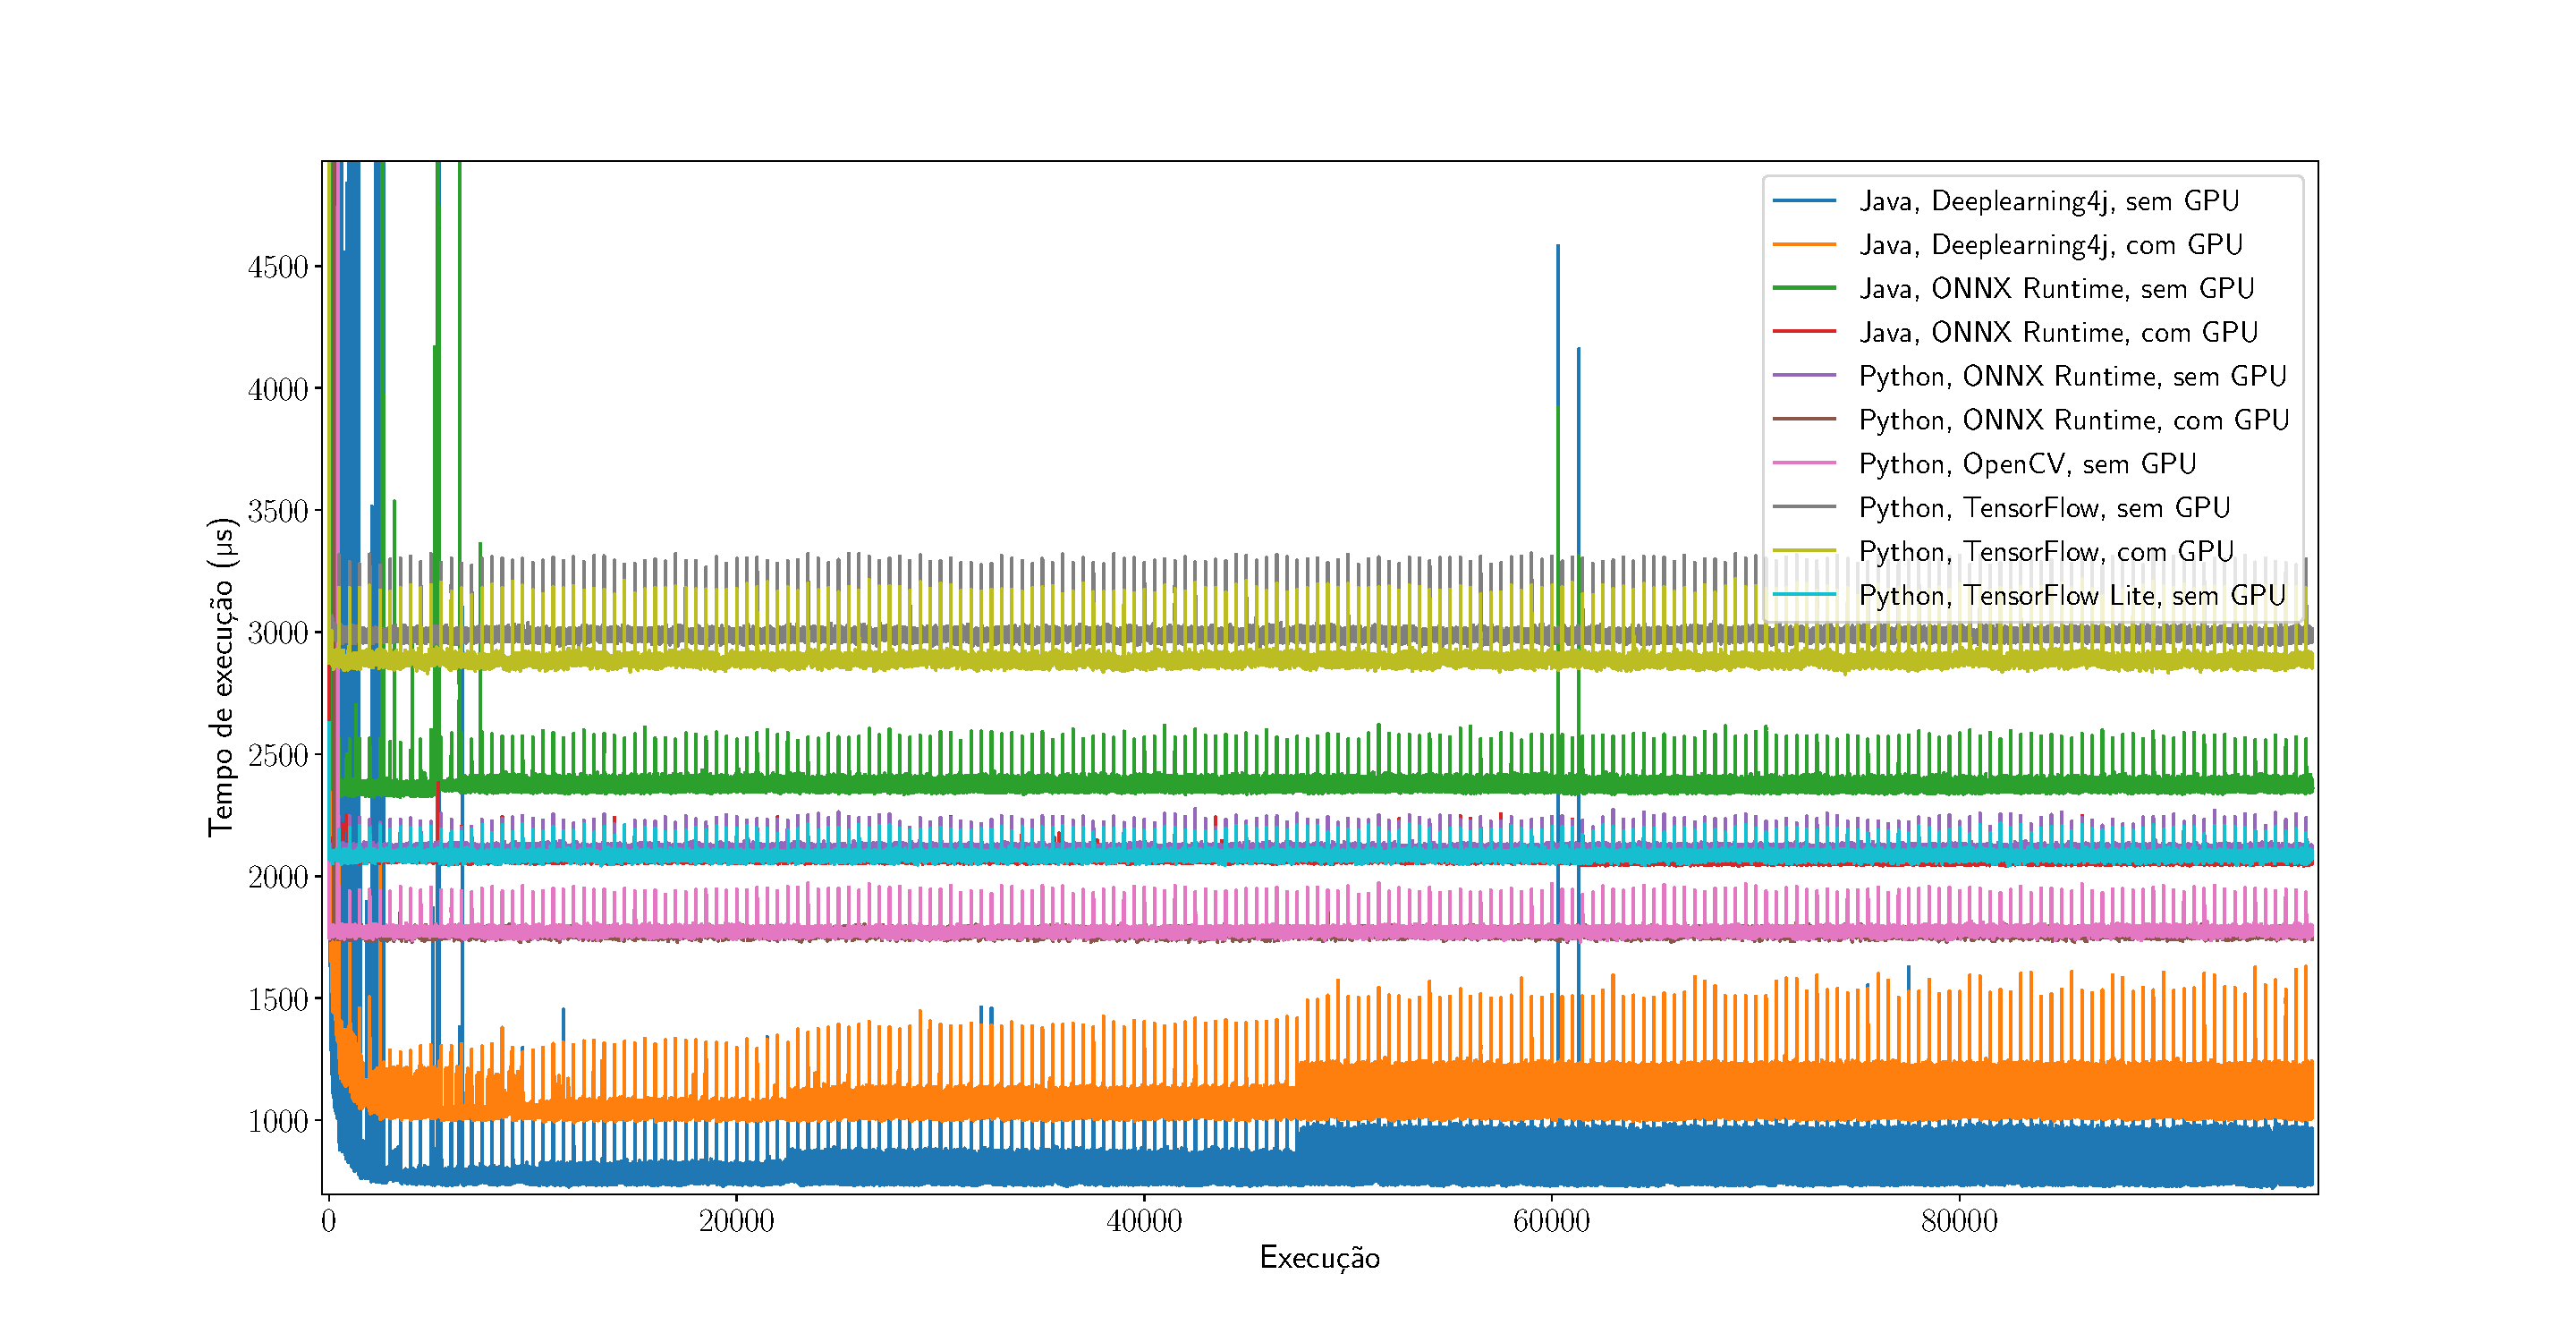
\includegraphics[width=\paperwidth]{img/all.pdf}}
  \caption{Tempo de execução de execuções sequenciais do modelo para cada programa de simulação}
  \label{fig:all}
\end{figure}